\documentclass[pdf]{beamer}
\mode<presentation>{} 

\usepackage{hyperref}
\usepackage{pgf}
\usepackage{fancyhdr}
\usepackage{tikz}
\usetikzlibrary{trees}
\usetikzlibrary{arrows,automata}
\usetikzlibrary{automata,positioning}
\usetikzlibrary{shapes}
\usepackage{tikz-qtree,tikz-qtree-compat}
\usepackage{mathtools,enumerate,amssymb}
\usetikzlibrary{patterns}
\usepackage[utf8]{inputenc}
\usepackage[T1]{fontenc}
\usepackage{graphicx}
\usepackage{varwidth}
\usepackage{xcolor}
\usepackage{multicol}
\usepackage{multirow}
\usepackage[export]{adjustbox}
\usepackage{wrapfig}
\usepackage{textcomp}
\usepackage{eso-pic}
\usepackage{pgfornament}
\usepackage[export]{adjustbox}



\newcommand\PlaceText[3]{%
\begin{tikzpicture}[remember picture,overlay]
\node[outer sep=0pt,inner sep=0pt,anchor=south west] 
  at ([xshift=#1,yshift=-#2]current page.north west) {#3};
\end{tikzpicture}%
}




\definecolor{background}{RGB}{255,255,255}
\setbeamercolor{background canvas}{bg=background}
\setbeamercolor{frametitle}{fg=blue}



\title{Representations and information visualization}
\subtitle{Human Computer Interaction}
\AtBeginSection[]{}



\setbeamertemplate{sidebar right}{}
\setbeamertemplate{footline}{%
\hfill\usebeamertemplate***{navigation symbols}
\hspace{1cm}\insertframenumber{}/\inserttotalframenumber}

\graphicspath{{./img/}}



\begin{document}



{\setbeamercolor{background canvas}{bg=background}
\begin{frame}
\vspace{10mm}
\huge{\raggedleft{\color{black}{\textbf{Representations and information visualization}}}}

\large{\raggedleft{\color{black} Human Computer Interaction}}

\begin{flushright}
\end{flushright}

\fontsize{7pt}{1pt}\selectfont{
Based on slide deck 

\textbf{Part 4: Designing and building visual interfaces. Representations and information visualization}

Human Computer Interaction I: Principles and Design

by

\textbf{Saul Greenberg}
\newline
Professor
\newline
\textbf{University of Calgary, Canada}

\textit{The new slides are marked with a *}
}

\fontsize{5pt}{1pt}\selectfont{ \textcolor{lightgray}
{Slide deck by Saul Greenberg. Permission is granted to use this for non-commercial purposes as long as general credit to Saul Greenberg is clearly maintained.
Warning: some material in this deck is used from other sources without permission. Credit to the original source is given if it is known.}}

\end{frame}}



% Inaintea codului fiecarui slide se vor scrie urmatoarele informatii:
% Nume si prenume student
% Numarul slide-ului corespunzator din prezentarea prof. Saul Greenberg
% Numele imaginilor inserate trebuie sa fie numar_slide_nume_imagine.extensie_imagine

%Tanasie Diana
%Numarul slide-ului: 1

\begin{frame}
	\bigskip
    \textbf{\LARGE Representations and \LARGE}
    \newline \vspace{25px}
    \textbf{\LARGE information visualization \LARGE}
   	
    \textbf{Characteristics of good representations}
    \newline
    \textbf{Information visualization}
    \begin{itemize}
        \item[]guidelines 
        \item[]visual information-seeking mantra
        \item[]techniques
    \end{itemize}
\end{frame}



%Tanasie Diana
%Numarul slide-ului: 3

\begin{frame}
{\textbf{Representations}}{\textcolor{red}{\rule{12cm}{1.2pt}}}

\textbf{Representations}
\begin{itemize}
\item[\textcolor{black}{•}] formal system or mapping by which information can be specified  (D. Marr)
\item[\textcolor{black}{•}] a sign system in that it stands for something other than its self
\end{itemize}
\textbf{for example:}
\begin{itemize}
\item[] decimal: 34
\item[] binary: 100010
\item[] roman: XXXIV
\end{itemize}
\textbf{different representations reveal different aspects of the information}
\begin{itemize}
\item[] decimal: counting \& information about powers of 10
\item[] binary: counting \& information about powers of 2
\item[] roman: counting
\end{itemize}
\textbf{Presentation}
\begin{itemize}
\item[] how the representation is placed or organized on the screen 
\item[] \textsl{\textcolor{red}{\LARGE 34 \LARGE} } , { \textcolor{blue}{\LARGE \textbf{34}   \LARGE}, \textcolor{black}{\LARGE \underline{34} \LARGE}}
\end{itemize}

\AddToShipoutPictureFG*{
    \AtPageLowerLeft{
      \put(-2,2){
        \makebox[\paperwidth][r]{\fontsize{4pt}			{1pt}\selectfont{\color{gray}{Saul Greenberg}}}
      }
    }  
}

\end{frame}



%Tanasie Diana
%Numarul slide-ului: 2

\begin{frame}
{\textbf{Representations - Good Representations}}{\textcolor{red}{\rule{12cm}{1.2pt}}}

{captures essential elements of the event / world}
\newline 
{deliberately leaves out / mutes the irrelevant}
\newline 
{appropriate for the person and their interpretation}
\newline 
{appropriate for the task, enhancing judgement ability}

\bigskip
\textbf{\large How many buffalo?   \qquad \qquad  \qquad  \qquad \qquad } \textbf{8}  \qquad \textbf{4}
\begin{picture}(0,0)
      \put(-55,70){\hbox{
\includegraphics[scale=0.5]{2_picture3.png}}}
\end{picture}
\begin{picture}(0,0)
      \put(-55,35){\hbox{
\includegraphics[scale=0.5]{2_picture4.png}}}
\end{picture}
\begin{picture}(0,0)
      \put(-55,5){\hbox{
\includegraphics[scale=0.5]{2_picture5.png}}}
\end{picture}
\begin{picture}(0,0)
      \put(-300,-120){\hbox{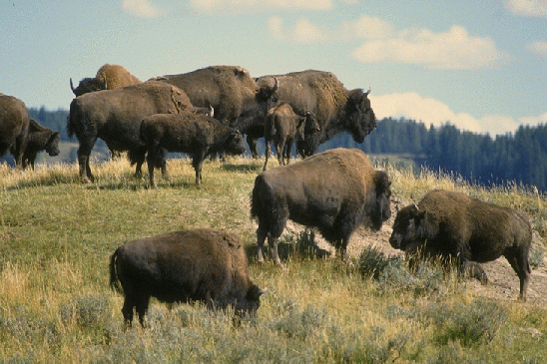
\includegraphics[scale=0.4]{2_picture1.png}}}
\end{picture}
\begin{picture}(0,0)
      \put(-120,-120){\hbox{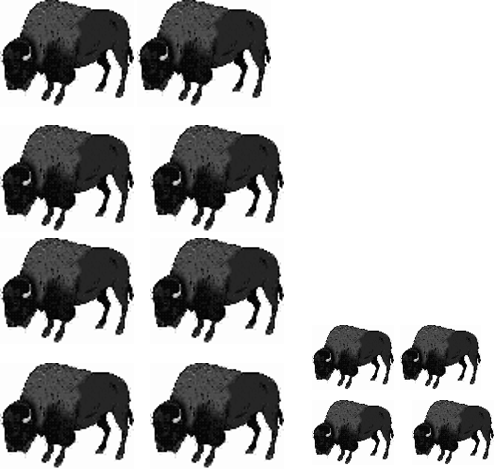
\includegraphics[scale=0.4]{2_picture2.png}}}
\end{picture}
\newline
\newline
\vspace{120px}

\AddToShipoutPictureFG*{
    \AtPageLowerLeft{
      \put(-2,2){
        \makebox[\paperwidth][r]{\fontsize{4pt}			{1pt}\selectfont{\color{gray}{Saul Greenberg}}}
      }
    }  
}
    
\end{frame}



%Tomei Alexandru
%Numarul slide-ului: 4

\begin{frame}
{\textbf{Representations - Mayan Numerals}}{\textcolor{red}{\rule{12cm}{1.2pt}}}

\begin{picture}(0,0)
	\put(-20,39){\hbox{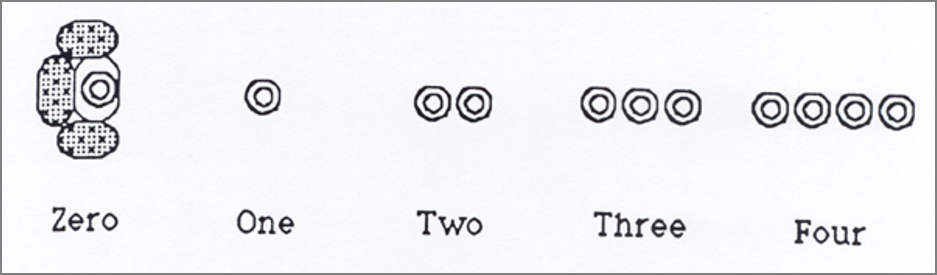
\includegraphics[scale=0.4]{4_Picture1.png}}}
\end{picture}
\begin{picture}(0,0)
	\put(15,-17){\hbox{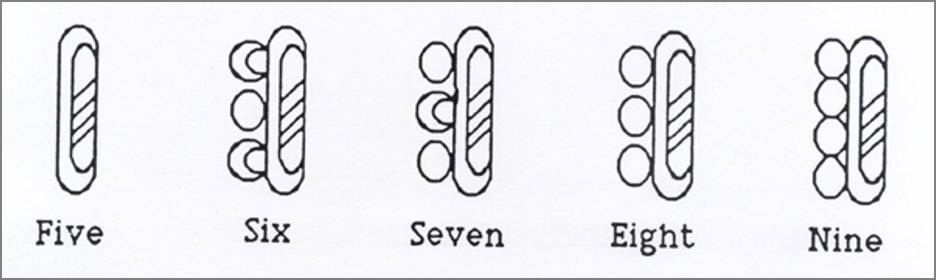
\includegraphics[scale=0.4]{4_Picture2.png}}}
\end{picture}
\begin{picture}(0,0)
	\put(55,-74){\hbox{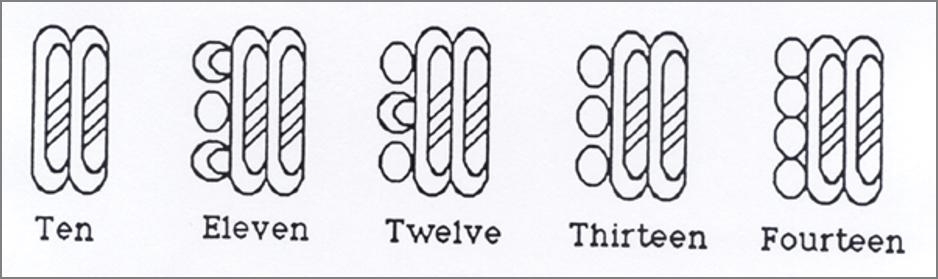
\includegraphics[scale=0.4]{4_Picture3.png}}}
\end{picture}
\begin{picture}(0,0)
	\put(100,-130){\hbox{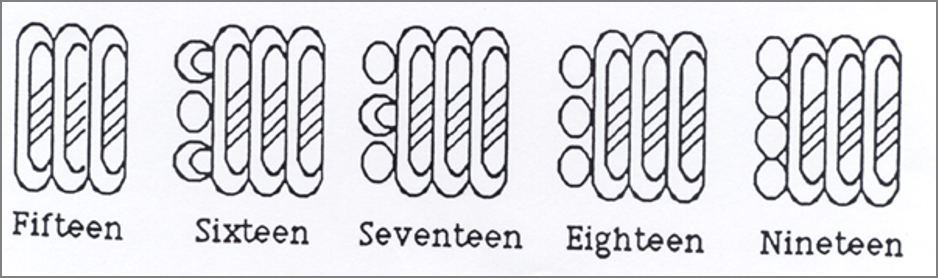
\includegraphics[scale=0.4]{4_Picture4.png}}}
\end{picture}
\end{frame}



%Tomei Alexandru
%Numarul slide-ului: 5

\begin{frame}
{\textbf{Representations - Egyptian Numerals}}{\textcolor{red}{\rule{12cm}{1.2pt}}}

\begin{picture}(0,0)
	\put(-20,39){\hbox{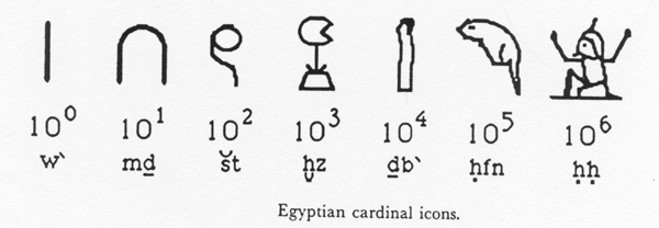
\includegraphics[scale=0.5]{5_Picture1.jpg}}}
\end{picture}
\begin{picture}(0,0)
	\put(52,-6){\hbox{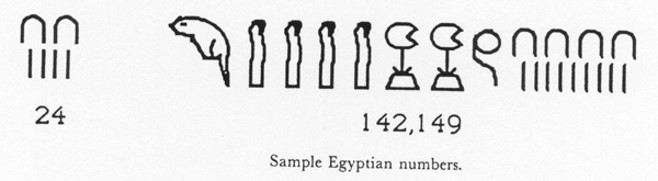
\includegraphics[scale=0.5]{5_Picture2.jpg}}}
\end{picture}
\begin{picture}(0,0)
	\put(140,-88){\hbox{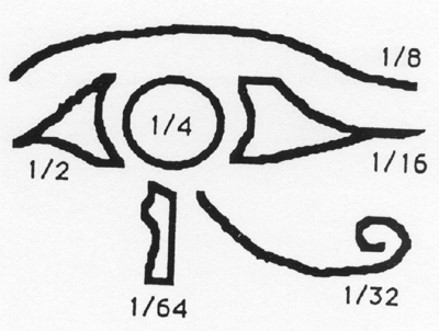
\includegraphics[scale=0.5]{5_Picture3.jpg}}}
\end{picture}
\begin{picture}(0,0)
	\put(165,-141){\hbox{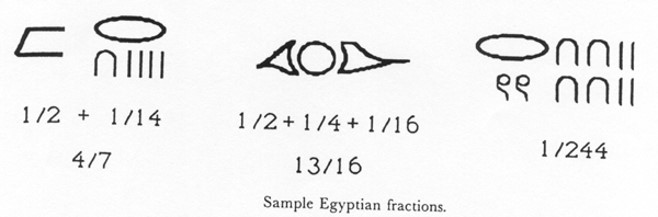
\includegraphics[scale=0.5]{5_Picture4.jpg}}}
\end{picture}
\end{frame}



%Tomei Alexandru
%Numarul slide-ului: 6

\begin{frame}
{\textbf{Representations}}{\textcolor{red}{\rule{12cm}{1.2pt}}}

{\textbf{\large Solving a problem simply means representing it so as to make the solution transparent }}
\begin{align*}
{\textrm{\qquad \qquad \qquad \qquad \qquad \qquad \qquad \qquad \qquad \qquad (Simon, 1981)}}
\end{align*}
\newline
\newline
\newline
{\textbf{\large Good representations \large}}
\begin{itemize}
\item[{-}] {allow people to find relevant information} 
\begin{itemize}
\item[{•}] {information may be present but hard to find}
\end{itemize}
\item[]
\item[{-}] {allow people to compute desired conclusions} 
\begin{itemize}
\item[{•}] {computations may be difficult or "for free" depending on representations} 
\end{itemize}
\end{itemize}
    \AddToShipoutPictureFG*{
    \AtPageLowerLeft{\put(-2,2){\makebox[\paperwidth][r]{\fontsize{4pt}{1pt}\selectfont{\color{gray}{Saul Greenberg}}}}}  
    }
\end{frame}



%Tomei Alexandru
%Numarul slide-ului: 7
\newcommand{\linie}[6]{
\begin{tikzpicture}
\draw[draw=#1,line width=#2] (#3,#4) -- +(#5,#6) ;
\end{tikzpicture}
}
\begin{frame}
{\textbf{Which is the best flight?}}{\textcolor{red}{\rule{12cm}{1.2pt}}}

\leavevmode\makebox(0,0){\put(-20,130){{\LARGE lenght \LARGE}}
\put(-20,110){{\LARGE stop-overs \LARGE}}
\put(-20,90){{\LARGE switches ... \LARGE}}}

\leavevmode\makebox(0,0){\put(100,142){
\renewcommand{\arraystretch}{0.7}
\begin{tabular}{ c c c c }
 \space & \space & \textrm{\scriptsize depart} & \textrm{\scriptsize arrive}\\
 \scriptsize 117 & \scriptsize Vancouver-Calgary & \scriptsize 7:00 & \scriptsize 9:00\\  
 \scriptsize Cdn 321 & \scriptsize Vancouver-Calgary & \scriptsize 9:00 & \scriptsize 12:00\\
 \scriptsize Cdn 355 & \scriptsize Calgary-Montreal & \scriptsize 13:30 & \scriptsize 19:30\\
 \scriptsize AC 123 & \scriptsize Calgary-Toronto & \scriptsize 12:30 & \scriptsize 16:30\\
 \scriptsize Ac 123 & \scriptsize Toronto-Montreal & \scriptsize 16:45 & \scriptsize 17:30\\
 \tiny *time zone: &  \tiny +1 van-cal, & \tiny +2 cal-tor, & \tiny mtl   \\
\end{tabular}
}}

\vspace{5px}
\hspace{155px}
\begin{picture}(0,0)
%%%%tabel
\put(0,0){\linie{gray}{0.8}{0}{0}{4.66}{0}}
\put(0,-100){\linie{gray}{0.8}{0}{0}{4.66}{0}}
\put(0,-120){\linie{gray}{0.8}{0}{0}{0}{5}}
\put(12,-120){\linie{gray}{0.8}{0}{0}{0}{5}}
\put(24,-120){\linie{gray}{0.8}{0}{0}{0}{5}}
\put(36,-120){\linie{gray}{0.8}{0}{0}{0}{5}}
\put(48,-120){\linie{gray}{0.8}{0}{0}{0}{5}}
\put(60,-120){\linie{gray}{0.8}{0}{0}{0}{5}}
\put(72,-120){\linie{gray}{0.8}{0}{0}{0}{5}}
\put(84,-120){\linie{gray}{0.8}{0}{0}{0}{5}}
\put(96,-120){\linie{gray}{0.8}{0}{0}{0}{5}}
\put(108,-120){\linie{gray}{0.8}{0}{0}{0}{5}}
\put(120,-120){\linie{gray}{0.8}{0}{0}{0}{5}}
\put(132,-120){\linie{gray}{0.8}{0}{0}{0}{5}}

%%%linii
\put(0,0){\linie{blue}{1}{0}{0}{0.4}{-0.78}}
\put(24,0){\linie{red}{1}{0}{0}{0.85}{-0.78}}
\put(48,-100){\linie{blue}{1}{0}{0}{1}{-3.54}}
\put(65,-120){\linie{red}{1}{0}{0}{1.7}{-4.2}}
\put(85,-120){\linie{blue}{1}{0}{0}{0.2}{-0.72}}
\put(77,-100){\linie{blue}{1}{0}{0}{0.3}{0}}
\end{picture}

%%Texte tabel
\leavevmode\makebox(0,0){\put(162,80){\tiny 7 \hspace{16px} 9 \hspace{13px} 11 \hspace{13px} 13 \hspace{13px} 15 \hspace{13px} 17 }}
\leavevmode\makebox(0,0){\put(155,20){\tiny 8 \hspace{16px} 10 \hspace{13px} 12 \hspace{13px} 14 \hspace{13px} 16 \hspace{13px} 18 }}
\leavevmode\makebox(0,0){\put(150,-225){\tiny 10 \hspace{13px} 12 \hspace{13px} 14 \hspace{13px} 16 \hspace{13px} 18 \hspace{13px} 20 }}

\leavevmode\makebox(0,0){
\put(115,-55){\scriptsize Vancouver }
\put(119,-75){\scriptsize Calgary }
\put(117,-175){\scriptsize Toronto }
\put(116,-195){\scriptsize Montreal }
}
\leavevmode\makebox(0,0){
\put(138,75){\tiny AC 117 }
\put(190,75){\textit{\tiny Cdn 321} }}
\leavevmode\makebox(0,0){
\put(199,-78){\textit{\tiny AC 123 }}
\put(240,-75){\textit{\tiny Cdn 355}}} 
    \AddToShipoutPictureFG*{
    \AtPageLowerLeft{\put(-2,2){\makebox[\paperwidth][r]{\fontsize{4pt}{1pt}\selectfont{\color{gray}{Saul Greenberg}}}}}  
    }    
\end{frame}



%Tomei Alexandru
%Numarul slide-ului: 8

\begin{frame}
{\textbf{When do I take my drugs?}}{\textcolor{red}{\rule{12cm}{1.2pt}}}

\leavevmode\makebox(0,0){\put(-20,130){{\large 10 - 30\% error rate in taking pills, same for pillbox organizers}}}

\leavevmode\makebox(0,0){
\put(-30,100){
\begin{tabular}{ c c }
 \space & \space \\ 
 {\scriptsize Inderal} & {\scriptsize - }\\  
 {\scriptsize Lanoxin} & {\scriptsize -} \\
 {\scriptsize Carafate} & {\scriptsize - }\\
 {\scriptsize Zantac} & {\scriptsize -} \\
 {\scriptsize Quinag} & {\scriptsize - }\\
 {\scriptsize Couma} & {\scriptsize - }\\
\end{tabular}}}

\leavevmode\makebox(0,0){
\put(40,140){\textcolor{blue}{\scriptsize 1 tablet 3 times a day}}
\put(40,126){\textcolor{blue}{\scriptsize 1 tablet every a.m.}}
\put(40,112){\textcolor{blue}{\scriptsize 1 tablet before meals and at bedtime}}
\put(40,98){\textcolor{blue}{\scriptsize 1 tablet every 12 hours (twice a day)}}
\put(40,83){\textcolor{blue}{\scriptsize 1 tablet 4 times a day}}
\put(40,68){\textcolor{blue}{\scriptsize 1 tablet a day}}}

\leavevmode\makebox(0,0){\put(-30,-160){
\begin{tabular}{ c c c c c }
 \space & \scriptsize Breakfast & \scriptsize Lunch & \scriptsize Dinner & \scriptsize Bedtime \\ 
 \small Lanoxin & \tiny O & \space & \space & \space\\  
 \hline
 \small Inderal & \tiny O & \tiny O & \tiny O & \tiny O\\
 \hline
 \small Quinag & \tiny O & \tiny O & \tiny O & \tiny O\\
 \hline
 \small Carafate & \tiny O & \tiny O & \tiny O & \tiny O\\
 \hline
 \small Zantac & \space & \tiny O & \space & \tiny O\\
 \hline
 \small Couma &  \space & \space & \space & \tiny O   \\
\end{tabular}}}

\leavevmode\makebox(0,0){\put(175,-130){
\begin{tabular}{ c c c c }
 \scriptsize Breakfast & \scriptsize Lunch & \scriptsize Dinner & \scriptsize Bedtime \\ 
 \tiny Lanoxin & \tiny & \tiny & \tiny \\  
 \tiny Inderal & \tiny Inderal & \tiny Inderal & \tiny Inderal \\
 \tiny Quinag & \tiny Quinag & \tiny Quinag & \tiny Quinag \\
 \tiny Carafate & \tiny Carafate & \tiny Carafate & \tiny Carafate \\
 \space & \tiny Zantac & \space & \tiny Zantac \\
 \space &  \space & \space & \tiny Couma\\
\end{tabular}}}
   \AddToShipoutPictureFG*{
    \AtPageLowerLeft{\put(-280,2){\makebox[\paperwidth][r]{\fontsize{4pt}{1pt}\selectfont{\color{gray}{Adapted from Donald Norman}}}}}  
    }
    \AddToShipoutPictureFG*{
    \AtPageLowerLeft{\put(-2,2){\makebox[\paperwidth][r]{\fontsize{4pt}{1pt}\selectfont{\color{gray}{Saul Greenberg}}}}}  
    }
\end{frame}



%Tomei Alexandru
%Numarul slide-ului: 9

\begin{frame}
{\textbf{Which representation is best?}}{\textcolor{red}{\rule{12cm}{1.2pt}}}

{\textbf{\large depends heavily on task \large}}
\begin{minipage}[t]{0.9\linewidth}
\begin{minipage}[t]{0.25\linewidth}
\begin{flushleft}
	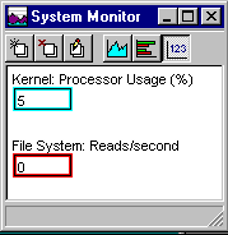
\includegraphics[scale=0.5]{9_Picture1.png}
    \newline
    \newline
    \newline
    \newline
    \newline
    \newline
    \newline
    \newline
    \newline
    \scriptsize What is precise value? \tiny
\end{flushleft}
\end{minipage}
\hfill
\begin{minipage}[t]{0.25\linewidth}
\begin{flushleft}
	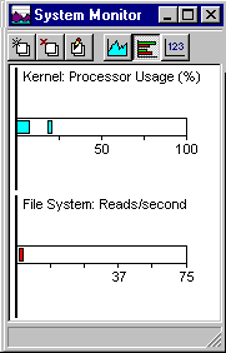
\includegraphics[scale=0.5]{9_Picture2.png}
    \newline
    \newline
    \scriptsize How does the performance now compared to its peak? 
\end{flushleft}
\end{minipage}
\hfill
\begin{minipage}[t]{0.25\linewidth}
\begin{flushleft}
	
\includegraphics[scale=0.5]{9_Picture3.png}
    \newline
    \newline
    \scriptsize How does the performance change over time?
\end{flushleft}
\end{minipage}
\end{minipage}
   \AddToShipoutPictureFG*{
    \AtPageLowerLeft{\put(-286,2){\makebox[\paperwidth][r]{\fontsize{4pt}{1pt}\selectfont{\color{gray}{Windows 95 System Monitor}}}}}  
    }
    \AddToShipoutPictureFG*{
    \AtPageLowerLeft{\put(-2,2){\makebox[\paperwidth][r]{\fontsize{4pt}{1pt}\selectfont{\color{gray}{Saul Greenberg}}}}}  
    }
\end{frame}



%Tomei Alexandru
%Numarul slide-ului: 10

\begin{frame}
{\textbf{Which folder has the most documents?}}{\textcolor{red}{\rule{12cm}{1.2pt}}}

\begin{picture}(0,0)
	\put(-20,0){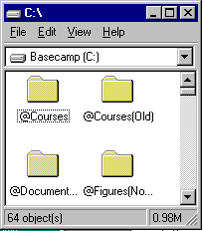
\includegraphics[scale=0.5]{10_Picture1.png}}
\end{picture}
\begin{picture}(0,0)
	\put(-23,-100){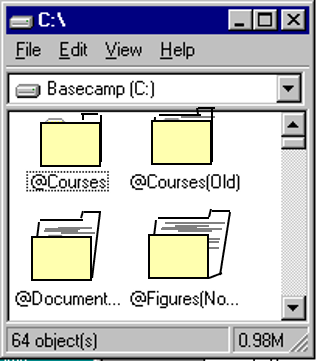
\includegraphics[scale=0.5]{10_Picture2.png}}
\end{picture}
\begin{picture}(0,0)
	\put(70,-40){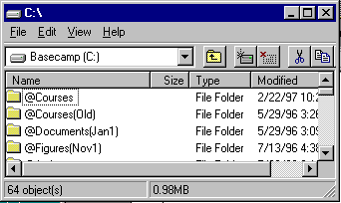
\includegraphics[scale=0.5]{10_Picture3.png}}
\end{picture}
\begin{picture}(0,0)
	\put(170,-45){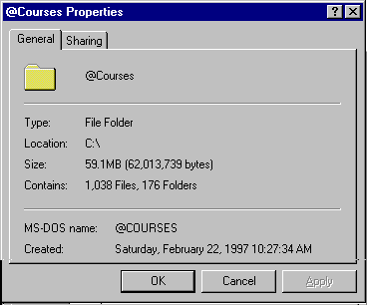
\includegraphics[scale=0.5]{10_Picture4.png}}
\end{picture}
\begin{picture}(0,0)
	\put(100,0){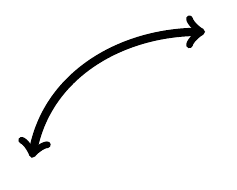
\begin{tikzpicture}
		\draw [<->,black,line width=3] (0,0) to [out=80,in=-180] (2.2,1.6);
	\end{tikzpicture}}
\end{picture}
\leavevmode\makebox(0,0){\put(100,120){\tiny right menu \tiny}
\put(100,110){\tiny + properties \tiny}}
   \AddToShipoutPictureFG*{
    \AtPageLowerLeft{\put(-299,2){\makebox[\paperwidth][r]{\fontsize{4pt}{1pt}\selectfont{\color{gray}{Windows 95 File Viewer}}}}}  
    }
    \AddToShipoutPictureFG*{
    \AtPageLowerLeft{\put(-2,2){\makebox[\paperwidth][r]{\fontsize{4pt}{1pt}\selectfont{\color{gray}{Saul Greenberg}}}}}  
    }
\end{frame}



%Tomei Alexandru
%Numarul slide-ului: 11

\begin{frame}
{\textbf{Where am I?}}{\textcolor{red}{\rule{12cm}{1.2pt}}}
     
     \begin{picture}(0,0)
		\put(60,-120){
\includegraphics[scale=0.45]{11_Picture1.png}}
	\end{picture}
    \leavevmode\makebox(0,0){\put(-30,100){\small Detailed navigation \small}
    \put(-30, 90){\small plus precision \small}}
     \leavevmode\makebox(0,0){\put(10,-262){\small General navigation plus orientation \small}}
     \begin{picture}(0,0)
		\put(35,15){
\begin{tikzpicture}
			\draw [->,red,line width=3] (0,0) to (1,-0.7);
		\end{tikzpicture}}
	\end{picture}
    \begin{picture}(0,0)
		\put(145,-125){
\begin{tikzpicture}
			\draw [->,red,line width=3] (0,0) to (0.4,0.7);
		\end{tikzpicture}}
	\end{picture}
\leavevmode\makebox(0,0){\put(100,120){\tiny right menu \tiny}
\put(100,110){\tiny + properties \tiny}}
   \AddToShipoutPictureFG*{
    \AtPageLowerLeft{\put(-299,2){\makebox[\paperwidth][r]{\fontsize{4pt}{1pt}\selectfont{\color{gray}{Windows NT Hover Game}}}}}  
    }
    \AddToShipoutPictureFG*{
    \AtPageLowerLeft{\put(-2,2){\makebox[\paperwidth][r]{\fontsize{4pt}{1pt}\selectfont{\color{gray}{Saul Greenberg}}}}}  
    }
\end{frame}



% Ungureanu Cornel Cristian
% 12
% 12_Prezent.png
\definecolor{bluemarin}{RGB}{0,0,102}
\begin{frame}
{\textbf{Where am I?}}{\textcolor{red}{\rule{12cm}{1.2pt}}}

\vspace{-0.5cm}

	\begin{picture}(0,0)
		\put(10,-220){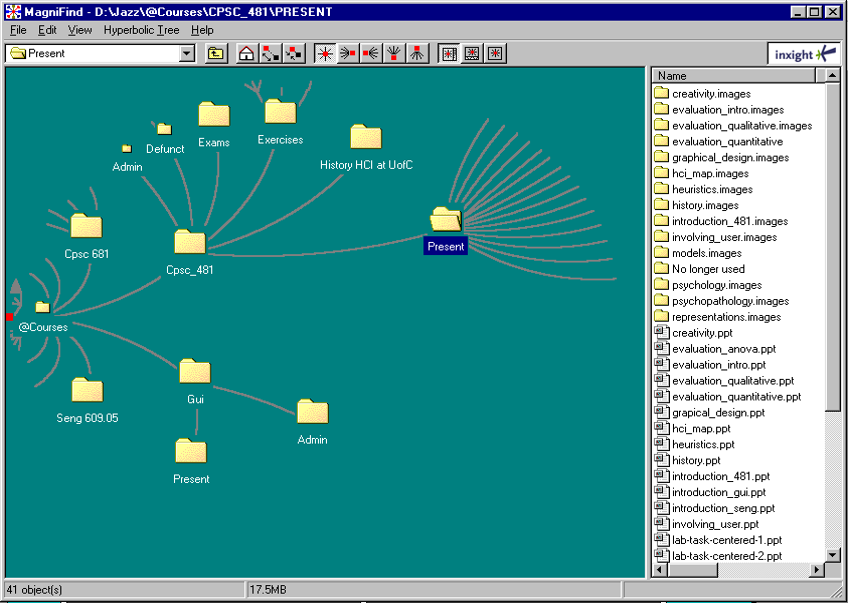
\includegraphics[scale=0.45]{12_Prezent.png}}
	\end{picture}
    \put(-25,-234){\tiny \color{gray}{Inxight Magnifind}}

\end{frame}



% Ungureanu Cornel Cristian
% 13
% 13_Saul_1.png
% 13_Saul_2.png

\begin{frame}
{\textbf{What do I have to do?}}{\textcolor{red}{\rule{12cm}{1.2pt}}}

\vspace{-0.4cm}

	\begin{picture}(0,0)
		\put(-20,-160){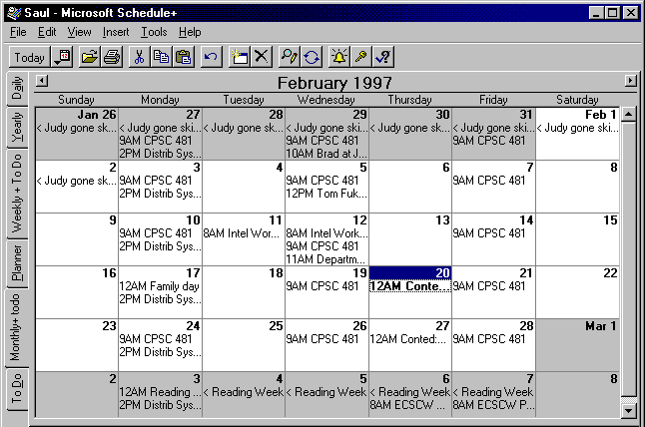
\includegraphics[scale=0.50]{13_Saul_1.png}}
	\end{picture}
    \begin{picture}(0,0)
		\put(110.5,-220){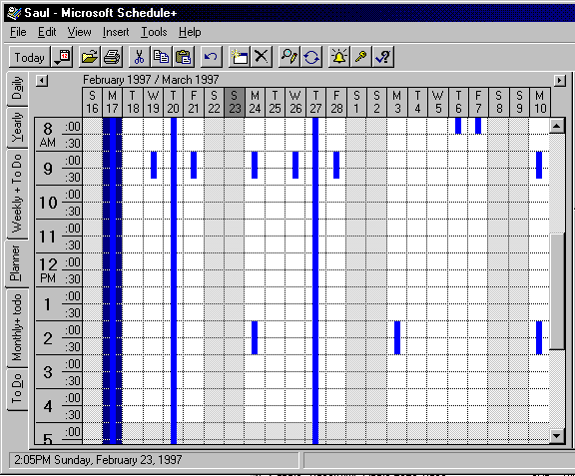
\includegraphics[scale=0.50]{13_Saul_2.png}}
	\end{picture}
	\put(-28,-234){\tiny \color{gray}{Microsoft Schedule+}}

\end{frame}



% Ungureanu Cornel Cristian
% 14

\begin{frame}
    {{\textbf{Information Visualization}}}{\textcolor{red}{\rule{12cm}{1.2pt}}}
    
    \Large Graphics should reveal the data
    \begin{itemize}
    \setlength{\baselineskip}{4mm}
	\item[\textcolor{black}{--}] {\normalsize show the data}
    \item[\textcolor{black}{--}] {\normalsize not get in the way of the message}
    \item[\textcolor{black}{--}] {\normalsize avoid distortion}
    \item[\textcolor{black}{--}] {\normalsize present many numbers in a small space}
    \item[\textcolor{black}{--}] {\normalsize make large data sets coherent}
    \item[\textcolor{black}{--}] {\normalsize encourage comparison between data}
    \item[\textcolor{black}{--}] {\normalsize supply both a broad overview and fine detail}
	\item[\textcolor{black}{--}] {\normalsize serve a clear purpose}
    \end{itemize}
    \begin{flushright}
    \setlength{\baselineskip}{0em}
    {\normalsize \itshape E. Tufte\\
    Visual Display of Quantitative Information}
    \end{flushright}
    \vfill
    \AddToShipoutPictureFG*{
    \AtPageLowerLeft{\put(-180,2){\makebox[\paperwidth][r]{\fontsize{5pt}{1pt}\selectfont{\color{gray}{many examples on the following slides are taken from Tufte's books}}}}}  
    }
    \AddToShipoutPictureFG*{
    \AtPageLowerLeft{\put(-2,2){\makebox[\paperwidth][r]{\fontsize{5pt}{1pt}\selectfont{\color{gray}{Saul Greenberg}}}}}  
    }
\end{frame}



% Ungureanu Cornel Cristian
% 15
% 15_tabela.png
% 15_LU.png
% 15_RU.png
% 15_LD.png
% 15_RD.png

\begin{frame}
    {{\textbf{*Anscombe’s Quartet}}}{\textcolor{red}{\rule{12cm}{1.2pt}}}

\begin{itemize}
\item comprises four datasets that have nearly identical simple descriptive statistics

\item yet appear \textbf{very different} when graphed

\item constructed in 1973 by the statistician Francis Anscombe to demonstrate the importance of graphing data before analysing it 
\end{itemize}
    
\url{https://en.wikipedia.org/wiki/Anscombe\%27s_quartet}

\end{frame}



\begin{frame}
    {{\textbf{*Anscombe’s Quartet}}}{\textcolor{red}{\rule{12cm}{1.2pt}}}

The data:

\begin{figure}
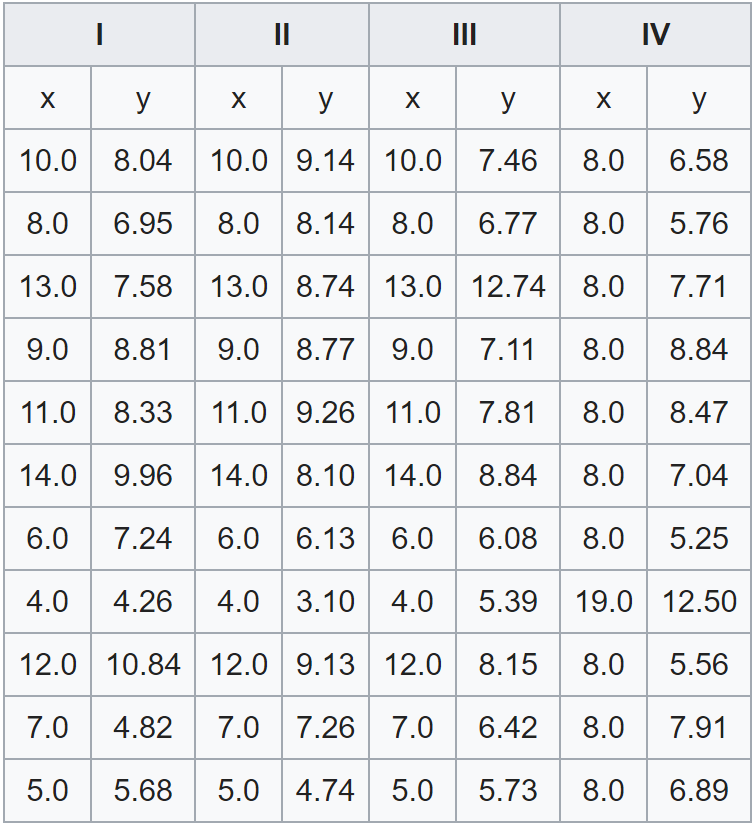
\includegraphics[scale=0.25]{15_Anscombe's_quartet_Data.png}
\end{figure}

\end{frame}



\begin{frame}
    {{\textbf{*Anscombe’s Quartet}}}{\textcolor{red}{\rule{12cm}{1.2pt}}}

For all four datasets the basic statistic properties are the same:
    
\begin{figure}
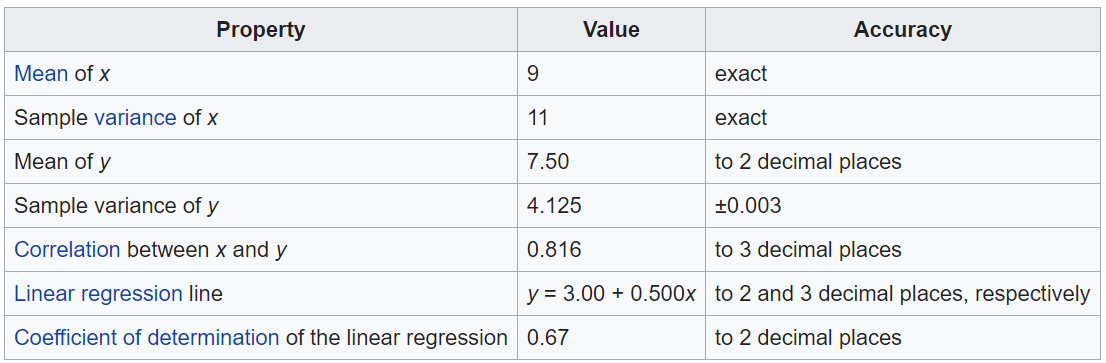
\includegraphics[scale=0.5]{15_Anscombe's_quartet_Prop.png}
\end{figure}

\end{frame}



\begin{frame}
    {{\textbf{Anscombe’s Quartet}}}{\textcolor{red}{\rule{12cm}{1.2pt}}}

But the \textbf{graphics reveal the data}:
    
\begin{figure}
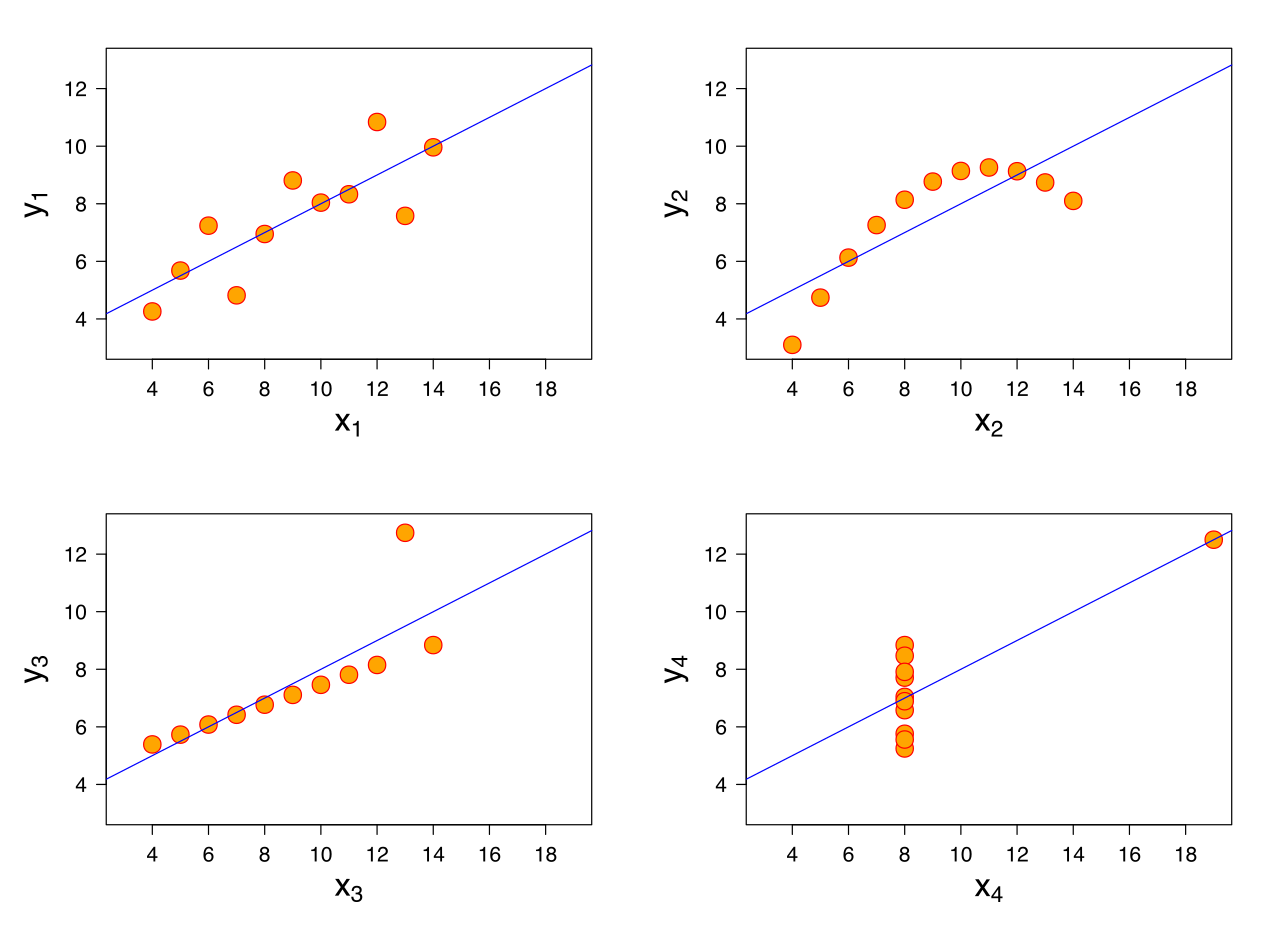
\includegraphics[scale=0.2]{15_Anscombe's_quartet.png}
\end{figure}

\end{frame}



% Ungureanu Cornel Cristian
% 16
% 16_tabel.png
% 16_graf.png
% 16_line.png
% 16_cerc.png

\begin{frame}
	{{\textbf{Do I deserve a tax break?}}}{\textcolor{red}{\rule{12cm}{1.2pt}}}
	
    \begin{picture}(0,0)
	\put(0,-125){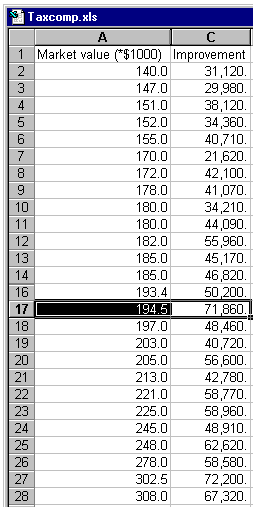
\includegraphics[scale=0.55]{16_tabel.png}}
\end{picture}
\begin{picture}(0,0)
	\put(107,-66){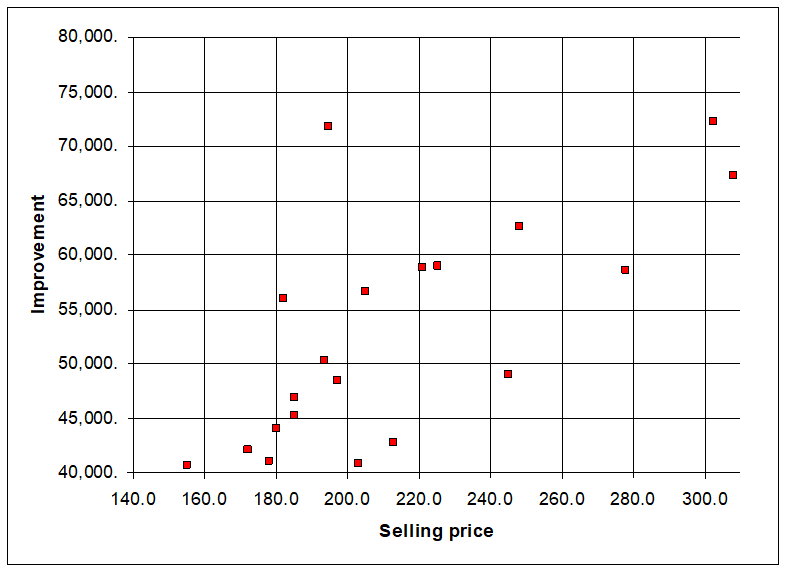
\includegraphics[scale=0.55]{16_graf.png}}
\end{picture}
\begin{picture}(0,0)
	\put(150,-41){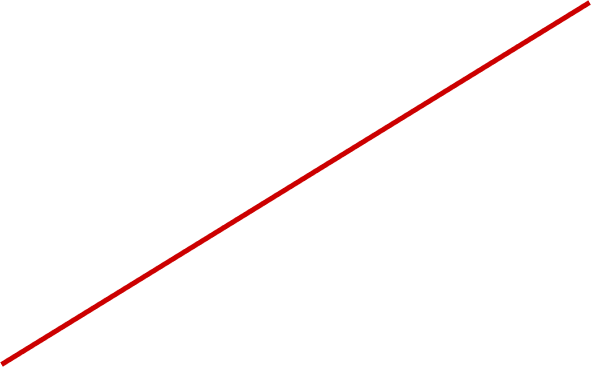
\includegraphics[scale=0.55]{16_line.png}}
\end{picture}
\begin{picture}(0,0)
	\put(178,42){
\includegraphics[scale=0.55]{16_cerc.png}}
\end{picture}
    \AddToShipoutPictureFG*{
    \AtPageLowerLeft{\put(-285,2){\makebox[\paperwidth][r]{\fontsize{4pt}{1pt}\selectfont{\color{gray}{Example by Saul Greenberg}}}}}  
    }
    \AddToShipoutPictureFG*{
    \AtPageLowerLeft{\put(-2,2){\makebox[\paperwidth][r]{\fontsize{4pt}{1pt}\selectfont{\color{gray}{Saul Greenberg}}}}}  
    }
\end{frame}



% Ungureanu Cornel Cristian
% 17
% 17_map.jpg

\begin{frame}
	{{\textbf{Exports of French Wine, 1864}}}{\textcolor{red}{\rule{12cm}{1.2pt}}}

    \begin{picture}(0,0)
		\put(-15,-120){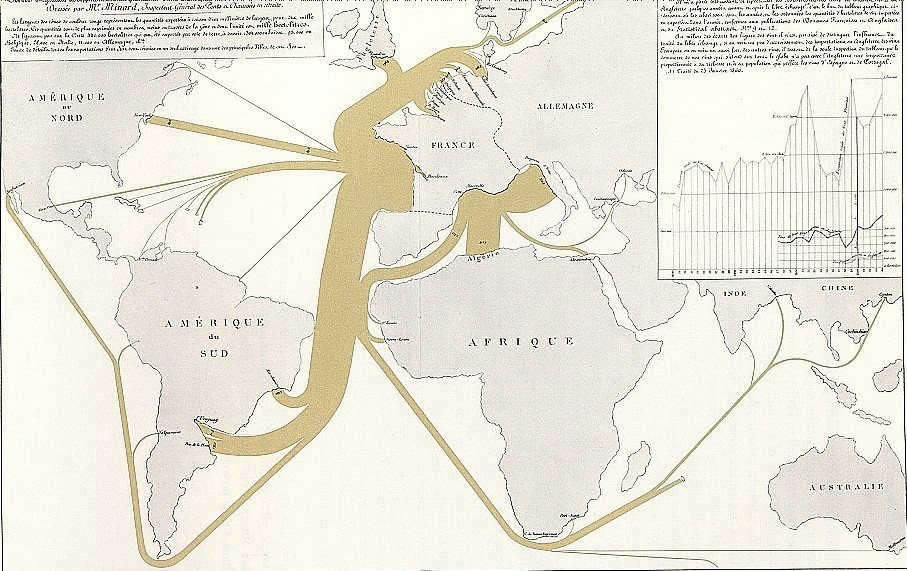
\includegraphics[scale=0.5]{17_map.jpg}}
	\end{picture}
    \AddToShipoutPictureFG*{
    \AtPageLowerLeft{\put(-200,2){\makebox[\paperwidth][r]{\fontsize{4pt}{1pt}\selectfont{\color{gray}{E. Tufte, "Visual Display of Quantitative Information"}}}}}  
    }
\end{frame}



% Ungureanu Cornel Cristian
% 18
% 18_Cholera.png
% 18_cerc.png
\begin{frame}
	{{\textbf{*Deaths by Cholera, Dr. John Snow, 1854}}}{\textcolor{red}{\rule{12cm}{1.2pt}}}
	
British doctor \textbf{John Snow} couldn't convince other doctors and scientists that cholera, a deadly disease, was spread when people drank contaminated water until a mother washed her baby's diaper in a town well in 1854 and touched off an epidemic that killed 616 people.
\newline

\url{https://www.ph.ucla.edu/epi/snow/snowcricketarticle.html}
\newline
	
\end{frame}



\begin{frame}
	{{\textbf{Deaths by Cholera, Dr. John Snow, 1854}}}{\textcolor{red}{\rule{12cm}{1.2pt}}}
	
\begin{figure}
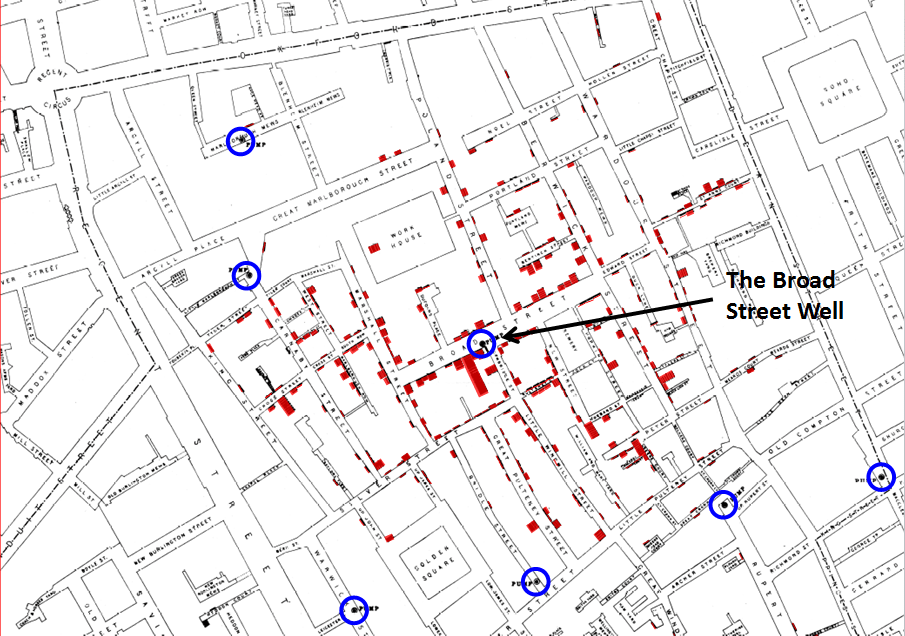
\includegraphics[scale=0.4]{18_Cholerafull_905.png}
\end{figure}

\end{frame}



\begin{frame}
	{{\textbf{*Deaths by Cholera, Dr. John Snow, 1854}}}{\textcolor{red}{\rule{12cm}{1.2pt}}}
		
\begin{itemize}
\item
in red his column of bars - each representing a cholera death

\item
in blue the local water pumps, including the Broad Street pump - servicing the well that was the source of cholera
\end{itemize}

\url{https://www.circleofblue.org/2013/world/peter-gleick-200-years-of-dr-john-snow-a-significant-figure-in-the-world-of-water/}

\end{frame}



% Ungureanu Cornel Cristian
% 19
% 19_march.png
% 19_cerc.png
\begin{frame}
	{{\textbf{*Napolean's march to Moscow, Charles Joseph Minard}}}{\textcolor{red}{\rule{12cm}{1.2pt}}}

The graphic is notable for its representation in two dimensions of six types of data:

\begin{itemize}
\item the number of Napoleon's troops

\item distance

\item temperature

\item the latitude and longitude

\item direction of travel

\item location relative to specific dates
\newline
\end{itemize}

\url{https://en.wikipedia.org/wiki/Charles_Joseph_Minard}

\end{frame}



\begin{frame}
	{{\textbf{Napolean's march to Moscow, Charles Joseph Minard}}}{\textcolor{red}{\rule{12cm}{1.2pt}}}

\begin{figure}
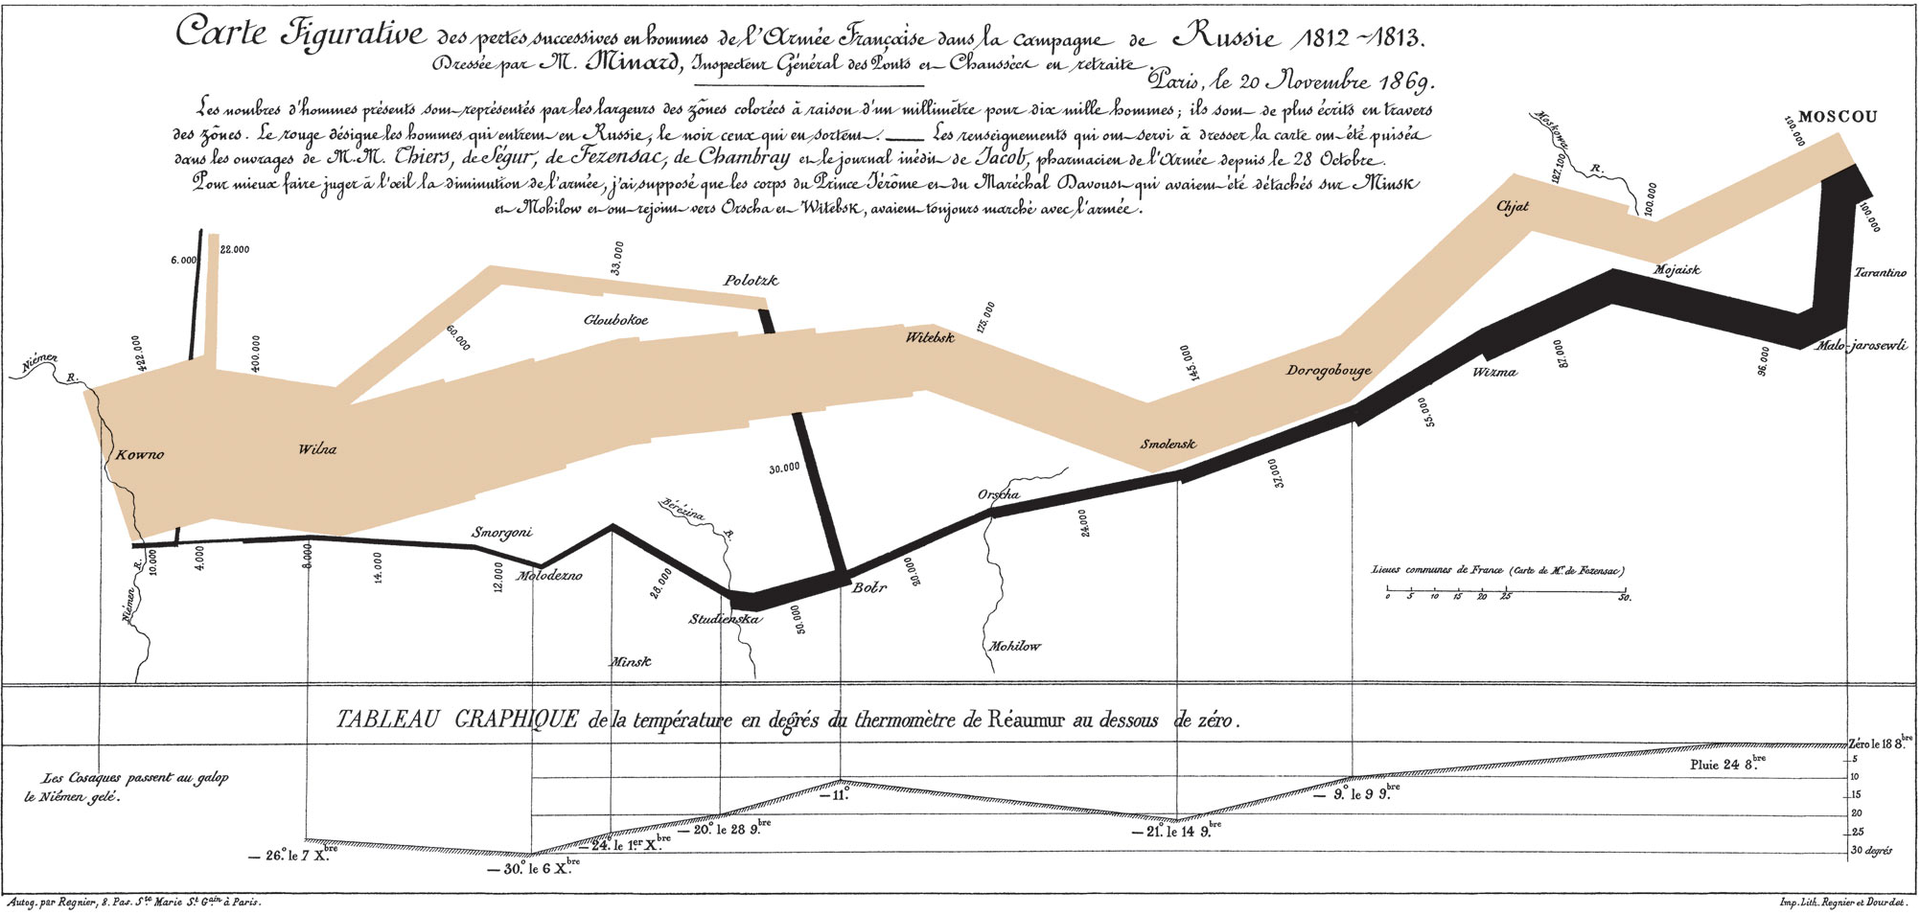
\includegraphics[scale=0.23]{19_Minard.png}
\end{figure}

\end{frame}



%Anghel Elena-Diana
%Numarul slide-ului: 20

\begin{frame}
    {\textbf{Chart Junk: A common error}}{\textcolor{red}{\rule{12cm}{1.2pt}}}
    
    \Large Information display is not just pretty graphics
    \begin{itemize}
    \item[\textcolor{black}{-}] {\large graphical re-design by amateurs on computers leads to "chart-junk", etc.}
    \end{itemize}
    \begin{picture}(0,0)
    \put(165,-140){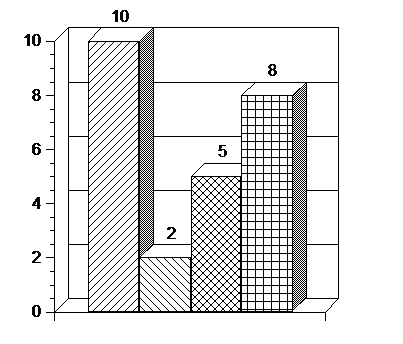
\includegraphics[scale=0.52]{20_Picture1.png}}
    \end{picture}
    \put(10,-40){\tiny Dear \textbf{Sir},}
    \put(10,-47){\underline{\tiny This is a \textit{really} \textbf{exciting} opportunity!}\scriptsize Take}
    \put(10,-56){\scriptsize advantage of it!}
    \put(290,-155){\tiny \color{gray}{Saul Greenberg}}
\end{frame}



%Anghel Elena-Diana
%Numarul slide-ului: 22

\begin{frame}
{\textbf{Chart Junk: \normalsize Removing deception and simplification}}{\textcolor{red}{\rule{12cm}{1.2pt}}}

\begin{picture}(0,0)
\put(-5,-100){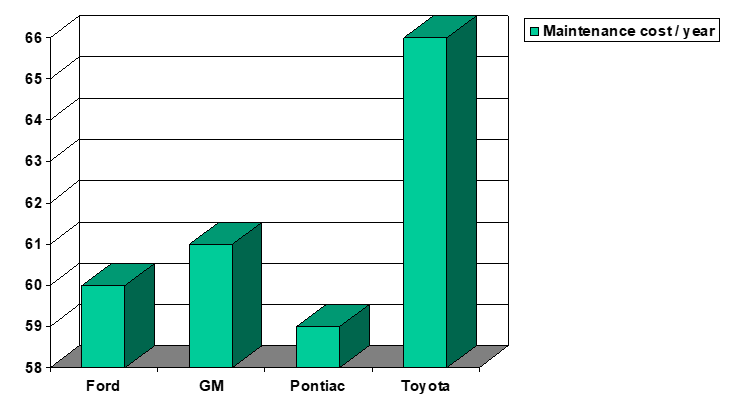
\includegraphics[scale=0.5]{22_Picture1.png}}
\end{picture}
\begin{picture}(0,0)
\put(165,-100){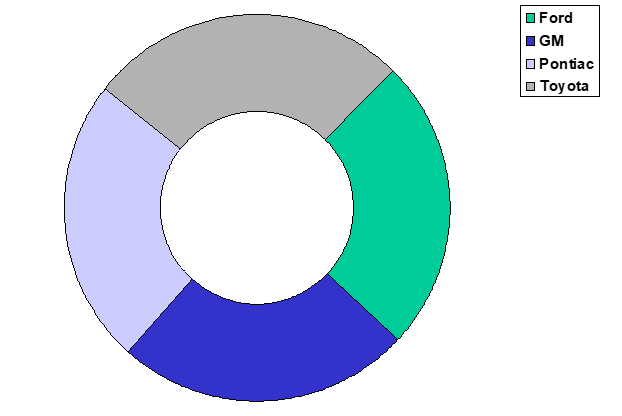
\includegraphics[scale=0.5]{22_Picture2.png}}
\end{picture}
\begin{picture}(0,0)
\put(-5,-215){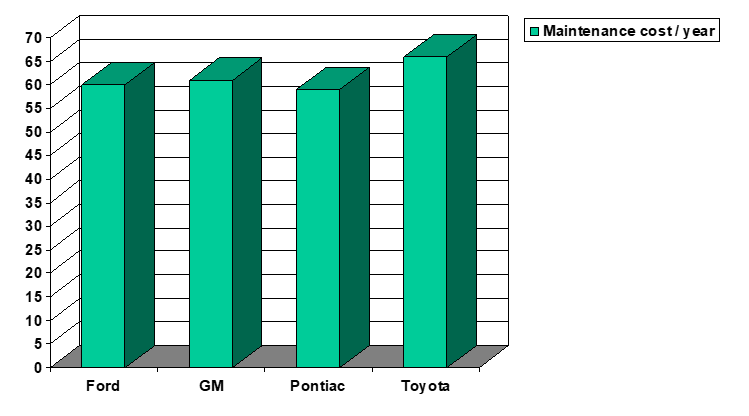
\includegraphics[scale=0.5]{22_Picture3.png}}
\end{picture}
\begin{picture}(0,0)
\put(170,-215){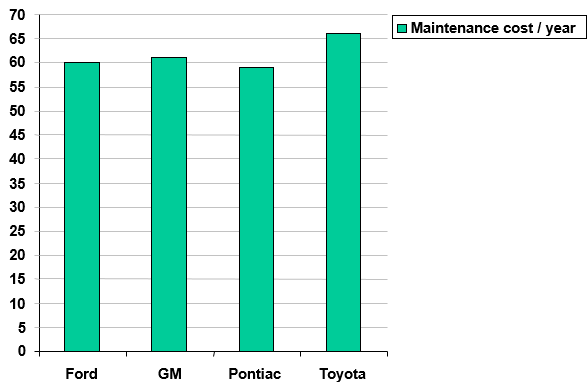
\includegraphics[scale=0.5]{22_Picture4.png}}
\end{picture}
\put(280,-223){\tiny \color{gray}{Saul Greenberg}}
\end{frame}



%Anghel Elena-Diana
%Numarul slide-ului: 24
\begin{frame}
{\textbf{*Small multiples}}{\textcolor{red}{\rule{12cm}{1.2pt}}}

\begin{itemize}
\item data visualization that consists of multiple charts arranged in a grid

\item it makes easy to compare the entirety of the data

\item a.k.a. trellis, lattice, grid, and panel charts
\newline
\end{itemize}

\url{https://www.displayr.com/what-are-small-multiples/}

\end{frame}



\begin{frame}
{\textbf{*Small multiples}}{\textcolor{red}{\rule{12cm}{1.2pt}}}

The required data for a small multiple is typically \textbf{a table}, where \textbf{the rows or columns contain the data for each of the separate series to be plotted}

\begin{figure}
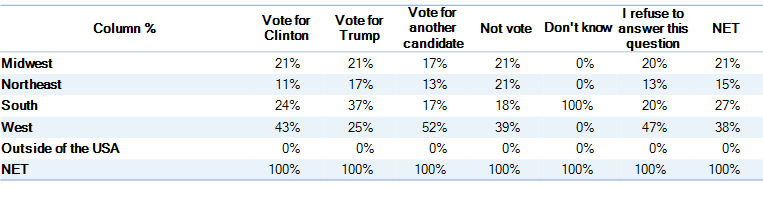
\includegraphics[scale=0.5]{24_SmallMultiple_Data.png}
\end{figure}

\end{frame}



\begin{frame}
{\textbf{*Small multiples}}{\textcolor{red}{\rule{12cm}{1.2pt}}}

\begin{figure}
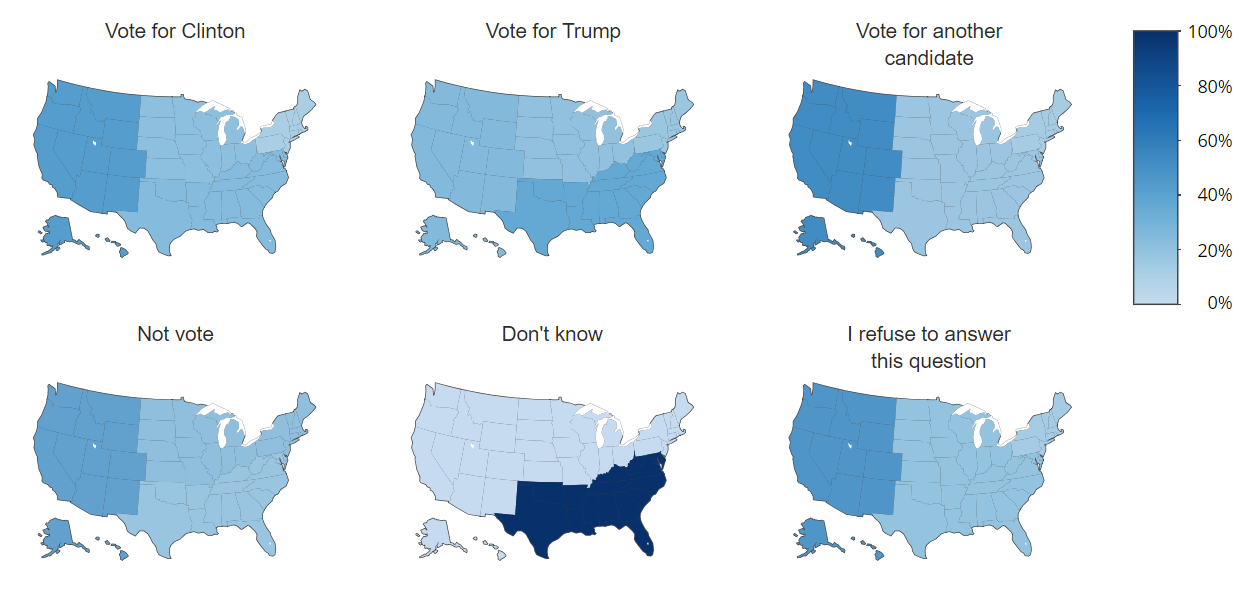
\includegraphics[scale=0.45]{24_SmallMultiple.png}
\end{figure}

\end{frame}



%Anghel Elena-Diana
%Numarul slide-ului: 27

\begin{frame}
{\textbf{Visual information-seeking mantra}}{\textcolor{red}{\rule{12cm}{1.2pt}}}

{\normalsize Overview first, zoom and filter, then details on demand}
\newline
{\normalsize Overview first, zoom and filter, then details on demand}
\newline
{\normalsize Overview first, zoom and filter, then details on demand}
\newline
{\normalsize Overview first, zoom and filter, then details on demand}
\newline
{\normalsize Overview first, zoom and filter, then details on demand}
\newline
{\normalsize Overview first, zoom and filter, then details on demand}
\newline
{\normalsize Overview first, zoom and filter, then details on demand}
\newline
{\normalsize Overview first, zoom and filter, then details on demand}
\newline
{\normalsize Overview first, zoom and filter, then details on demand}
\newline
{\normalsize Overview first, zoom and filter, then details on demand}
\newline
\newline
\put(25,0){ \small Shneiderman, Designing the User Interface 3rd Ed., 1997, p. 523 }
\put(290,-73){\tiny \color{gray}{Saul Greenberg}}
\end{frame}



%Ariton Elena-Gabriela
%Numarul slide-ului:29
%29_picture1.png
\begin{frame}
{\textbf{PhotoFinder}}{\textcolor{red}{\rule{12cm}{1.2pt}}}

\begin{figure}

\includegraphics[scale=0.45]{29_picture1.png}
\end{figure}
\end{frame}



\begin{frame}
{\textbf{*PhotoFinder}}{\textcolor{red}{\rule{12cm}{1.2pt}}}

University of Maryland, Human Computer Interaction Laboratory
\newline

\url{http://www.cs.umd.edu/hcil/photolib/}
\end{frame}



%Ariton Elena-Gabriela
%Numarul slide-ului:30
%30_picture1.png

\begin{frame}
{\textbf{Table Lens}}{\textcolor{red}{\rule{12cm}{1.2pt}}}

\vspace{-0.5cm}

    \begin{picture}(0,0)
		\put(10,-215){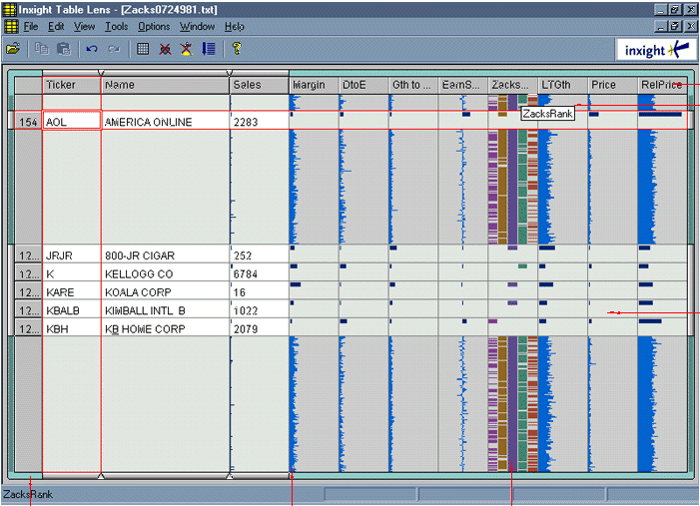
\includegraphics[scale=0.45]{30_picture1.png}}
	\end{picture}
	\put(-25,-225){\tiny \color{gray}{Inxight Table Lens
}} 
\end{frame}



%Ariton Elena-Gabriela
%Numarul slide-ului:31
%31_picture1.png

\begin{frame}
{\textbf{Table Lens}}{\textcolor{red}{\rule{12cm}{1.2pt}}}

\vspace{-0.3cm}

    \begin{picture}(0,0)
		\put(10,-215){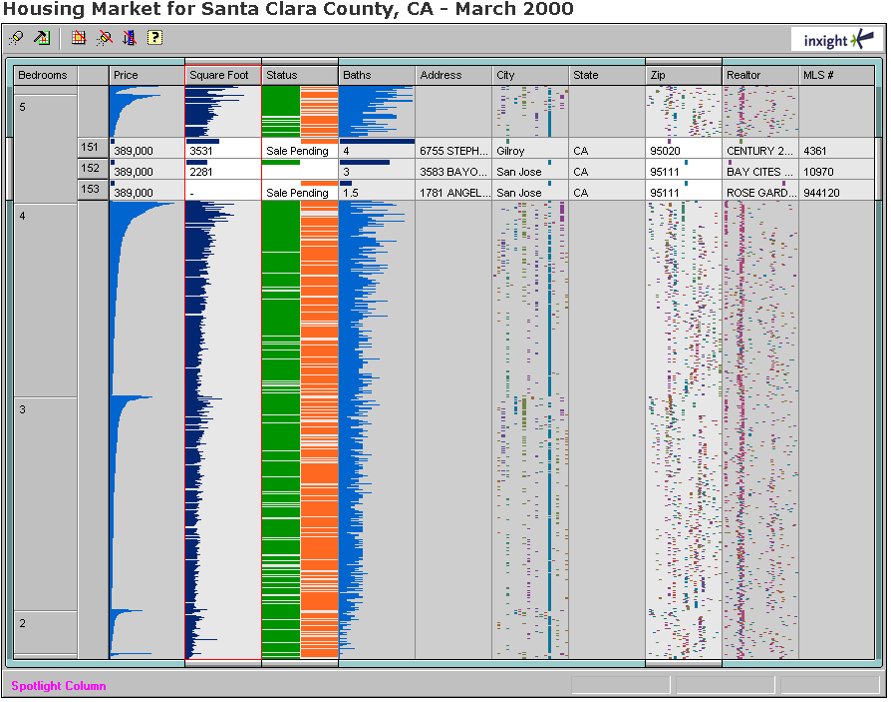
\includegraphics[scale=0.50]{31_picture1.png}}
	\end{picture}
	\put(-25,-225){\tiny \color{gray}{Inxight Table Lens
}} 
\end{frame}



\begin{frame}
{\textbf{*Table Lens}}{\textcolor{red}{\rule{12cm}{1.2pt}}}

Ramana Rao and Stuart K. Card, \textbf{The Table Lens: Merging Graphical and Symbolic Representations in an Interactive Focus+ Context Visualization for Tabular Information}, Proceedings of the SIGCHI conference on Human factors in computing systems, pp. 318-322, ACM, 1994
\newline

\url{http://citeseerx.ist.psu.edu/viewdoc/download?doi=10.1.1.115.8862&rep=rep1&type=pdf}

\end{frame}



%Ariton Elena-Gabriela
%Numarul slide-ului:32
%32_picture1.png
\begin{frame}
{\textbf{Infinite Zoom}}{\textcolor{red}{\rule{12cm}{1.2pt}}}

\begin{figure}
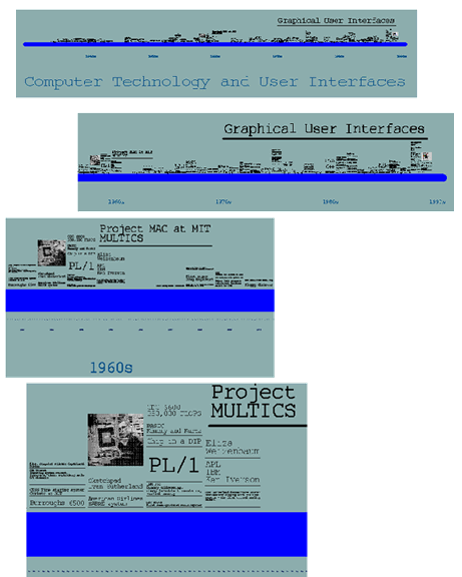
\includegraphics[scale=0.50]{32_picture1.png}
\end{figure}
\end{frame}



\begin{frame}
{\textbf{*Infinite Zoom}}{\textcolor{red}{\rule{12cm}{1.2pt}}}

B. B. Bederson et al, \textbf{Pad++: A Zoomable Graphical Sketchpad for Exploring Alternate Interface Physics}, Journal of Visual Languages and Computing vol. 7, issue 1, March 1996
\newline

\url{https://www.cs.umd.edu/hcil/pad++/papers/chi-94-pad/index.html}	
\newline

Article presentation:

\url{https://slideplayer.com/slide/8806742/}
	
\end{frame}



%Ariton Elena-Gabriela
%Numarul slide-ului:33
%33_picture1.png
\begin{frame}
{\textbf{Fisheye Menus}}{\textcolor{red}{\rule{12cm}{1.2pt}}}

\begin{figure}
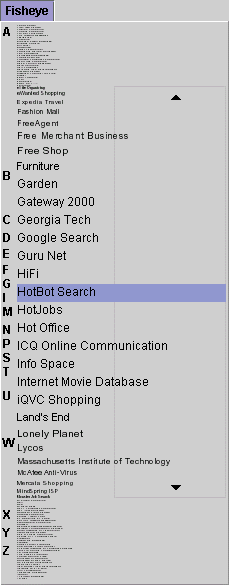
\includegraphics[scale=0.43]{33_fisheye_menu.png}
\end{figure}

\end{frame}



\begin{frame}
{\textbf{*Fisheye Menus}}{\textcolor{red}{\rule{12cm}{1.2pt}}}

B. B. Bederson, \textbf{Fisheye Menus}, Proceedings of ACM Conference on User Interface Software and Technology (UIST 2000), pp. 217-226, ACM Press, November 2000
\newline
    
\url{http://www.cs.umd.edu/hcil/fisheyemenu/}
\end{frame}



\begin{frame}
{\textbf{Fisheye Text Editors}}{\textcolor{red}{\rule{12cm}{1.2pt}}}

\begin{figure}
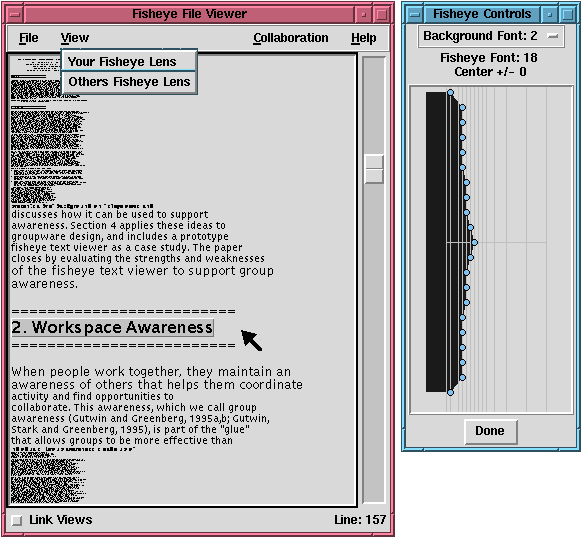
\includegraphics[scale=0.6]{34_fisheye_texta.png}
\end{figure}

\end{frame}



\begin{frame}
{\textbf{Fisheye Text Editors}}{\textcolor{red}{\rule{12cm}{1.2pt}}}

\begin{figure}
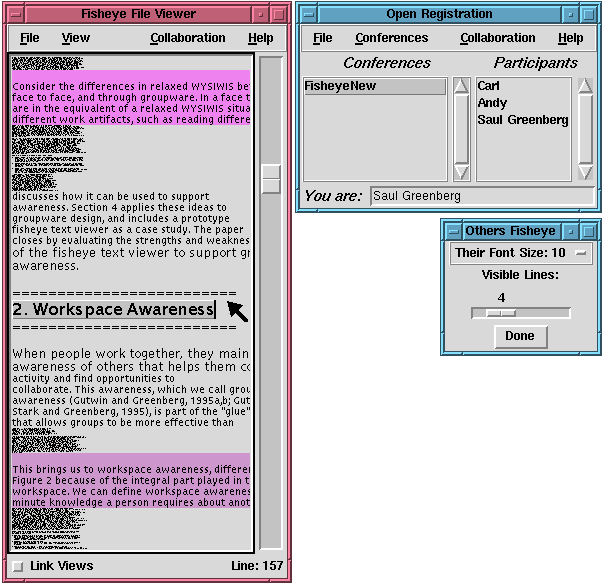
\includegraphics[scale=0.6]{34_fisheye_textb.png}
\end{figure}

\end{frame}



\begin{frame}
{\textbf{*Fisheye Text Editors}}{\textcolor{red}{\rule{12cm}{1.2pt}}}

Saul Greenberg, \textbf{A Fisheye Text Editor for Relaxed-WYSIWIS Groupware}, Conference on Human Factors in Computing Systems: Conference companion on Human factors in computing systems: common ground, vol. 13, no. 18, 1996
\newline
    
\url{http://citeseerx.ist.psu.edu/viewdoc/download?doi=10.1.1.41.4101&rep=rep1&type=pdf}
\end{frame}



%Ciobanu Iustin
%Numarul slide-ului:39

\begin{frame}
{\textbf{Perspective Wall}}{\textcolor{red}{\rule{12cm}{1.2pt}}}

\begin{figure}
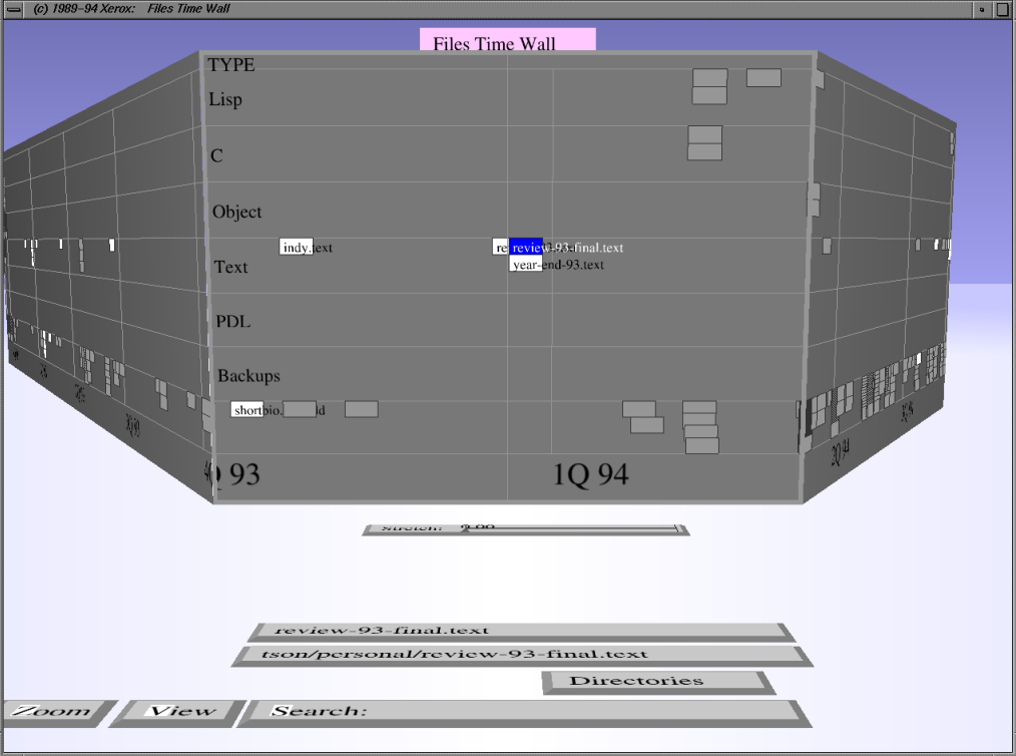
\includegraphics[scale=0.45]{39_Picture1.png}
\end{figure}

\end{frame}



\begin{frame}
{\textbf{Perspective Wall}}{\textcolor{red}{\rule{12cm}{1.2pt}}}

\begin{figure}
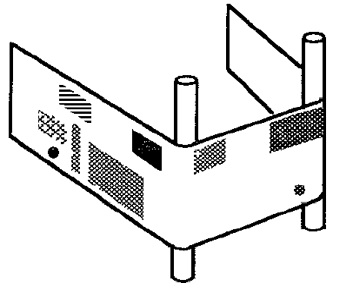
\includegraphics[scale=0.7]{39_Picture2.png}
\end{figure}

\end{frame}



\begin{frame}
{\textbf{*Perspective Wall}}{\textcolor{red}{\rule{12cm}{1.2pt}}}

Jock D. Mackinlay, George G. Robertson, Stuart K. Card, \textbf{The perspective wall: detail and context smoothly integrated}, CHI '91 Proceedings of the SIGCHI Conference on Human Factors in Computing Systems, pp. 173-176, New Orleans, Louisiana, USA, April 27 - May 02, 1991 
\newline

\url{https://www.researchgate.net/profile/Stuart_Card/publication/221514203_The_perspective_wall_Detail_and_context_smoothly_integrated/links/09e4150e317b65a315000000.pdf}

\end{frame}



%Ciobanu Iustin
%Numarul slide-ului:40

\begin{frame}
{\textbf{Document Lens}}{\textcolor{red}{\rule{12cm}{1.2pt}}}

\begin{figure}
\includegraphics[scale=0.5]{40_Picture1.png}
\end{figure}

\end{frame}



\begin{frame}
{\textbf{*Document Lens}}{\textcolor{red}{\rule{12cm}{1.2pt}}}

George G. Robertson, Jock D. Mackinlay, \textbf{The document lens}, UIST '93 Proceedings of the 6th annual ACM symposium on User interface software and technology, pp. 101-108, Atlanta, Georgia, USA 
\newline

\url{https://www.researchgate.net/profile/Jock_Mackinlay/publication/220877428_The_Document_Lens/links/0deec52598e6e183e0000000/The-Document-Lens.pdf}

\end{frame}



%Ciobanu Iustin
%Numarul slide-ului:41
\begin{frame}
{\textbf{Data Mountain}}{\textcolor{red}{\rule{12cm}{1.2pt}}}

\begin{figure}
\includegraphics[scale=0.45]{41_Picture2.png}
\end{figure}

\end{frame}



\begin{frame}
{\textbf{Data Mountain}}{\textcolor{red}{\rule{12cm}{1.2pt}}}

\begin{figure}
\includegraphics[scale=0.45]{41_Picture1.png}
\end{figure}

\end{frame}



\begin{frame}
{\textbf{*Data Mountain}}{\textcolor{red}{\rule{12cm}{1.2pt}}}

Robertson, Czerwinski, Larson, Robbins, Thiel, van Dantzich, \textbf{Data Mountain: Using Spatial Memory for Document Management}, Proceedings of the 11th annual ACM symposium on User interface software and technology, ACM, 1998
\newline

\url{http://www.academia.edu/download/43905411/Data_Mountain_Using_Spatial_Memory_for_D20160319-23716-bsl7qq.pdf}

\end{frame}



%Ciobanu Iustin
%Numarul slide-ului:42
\begin{frame}
{\textbf{Task Gallery}}{\textcolor{red}{\rule{12cm}{1.2pt}}}

\begin{figure}
\centering
\includegraphics[scale=0.45]{42_Picture1.png}
\end{figure}

\end{frame}



\begin{frame}
{\textbf{*Task Gallery}}{\textcolor{red}{\rule{12cm}{1.2pt}}}

George Robertson, Maarten van Dantzich, Daniel Robbins, Mary Czerwinski, Ken Hinckley, Kirsten Risden, David Thiel, Vadim Gorokhovsky, \textbf{The Task Gallery: A 3D Window Manager}, CHI '00 Proceedings of the SIGCHI conference on Human Factors in Computing Systems, April 2000
\newline

\url{https://www.microsoft.com/en-us/research/publication/the-task-gallery-a-3d-window-manager/}
\end{frame}



%Ciobanu Iustin
%Numarul slide-ului:43
\begin{frame}
{\textbf{Cone Trees}}{\textcolor{red}{\rule{12cm}{1.2pt}}}

\begin{figure}
\includegraphics[scale=0.4]{43_Picture1.png}
\end{figure}

\end{frame}



\begin{frame}
{\textbf{*Cone Trees}}{\textcolor{red}{\rule{12cm}{1.2pt}}}

Robertson, Mackinlay, \textbf{Cone Trees: Animated 3D Visualizations of Hierarchical Information}, CHI '91 Proceedings of the SIGCHI Conference on Human Factors in Computing Systems, pp. 189-194, New Orleans, Louisiana, USA, April 27 - May 02, 1991 
\newline

\url{https://www.researchgate.net/profile/Stuart_Card/publication/221515543_Cone_Trees_Animated_3D_Visualizations_of_Hierarchical_Information/links/09e4150e317b628c58000000.pdf}

\end{frame}



%Ciolacu Iulian-Teodor
%Numarul slide-ului: 44
\definecolor{textalbastru}{RGB}{0,0,102}
\definecolor{background}{RGB}{255,255,255}
\definecolor{blue}{RGB}{0,0,102}
\definecolor{background}{RGB}{255,255,255}
\begin{frame}
{\textbf{What you now know}}{\textcolor{red}{\rule{12cm}{1.2pt}}}

    \vspace{5px}
 \textcolor{blue}{ \fontsize{12}{20}\selectfont{Good representations}}
  \begin{itemize}
      	\item[--]\textcolor{blue}{ \fontsize{10}{0}\selectfont{appropriate for the person, their task, and their interpretation
}}
		\item[--]\textcolor{blue}{ \fontsize{10}{0}\selectfont{captures essential elements of the event / world \& mutes the irrelevant
}}
     \end{itemize}
 
 \vspace{5px}

 \textcolor{blue}{ \fontsize{12}{20}\selectfont{Information visualization}}
  \begin{itemize}
      	\item[--]\textcolor{textalbastru}{ \fontsize{10}{0}\selectfont{Tufte’s principles}}
        \item[--] \textcolor{textalbastru}{\fontsize{10}{0}\selectfont{overview first, zoom and filter, then details on demand}}
        \item[--]\textcolor{textalbastru}{ \fontsize{10}{0}\selectfont{many techniques now available}}
   \end{itemize}
   \vspace{80px}  
    \AddToShipoutPictureFG*{
    \AtPageLowerLeft{\put(-2,2){\makebox[\paperwidth][r]{\fontsize{4pt}{1pt}\selectfont{\color{gray}{Saul Greenberg}}}}}  
    }
\end{frame}



%%pt Slide-ul 47 ! Nu Sterge!!
\usetikzlibrary{arrows,positioning} 
\tikzset{
    %Define style for boxes
    punkt/.style={
           rectangle,
           draw=blue, thick,
           minimum height=2em,
           text centered},
    dreptunghi/.style={
           rectangle,
           draw=black,
           minimum height=2em}
}
\newcommand{\textbox}[5]{
\begin{tikzpicture}
\node[punkt,text width=#2] (market) {\textbf{#1}};
\draw[draw=blue] (market.north east)  +(0.2cm,-0.2) -- +(#3,-0.2cm) -- +(#4,#5) ;
\end{tikzpicture}
}

%Ciolacu Iulian-Teodor
%Numarul slide-ului: 47
\definecolor{textalbastru}{RGB}{0,0,102}
\definecolor{background}{RGB}{255,255,255}
\setbeamercolor{background canvas}{bg=background}

\newcommand{\sageatainsus}[7]{

\begin{tikzpicture}
        \node [single arrow,minimum width=#1, minimum height=#2,draw=black, rotate=#7,line width=#5,inner sep=#3] {   };
        \coordinate (P) at (0,0);
        \node[text width=#4] (N) at (P) {#6} ;
		
\end{tikzpicture}

}
\newcommand{\dreptunghi}[3]{

\begin{tikzpicture}
\node[dreptunghi,text width=#1,line width=#2] {#3};
\end{tikzpicture}

}
% culoare, grosime, lungime
\newcommand{\liniee}[3]{
\begin{tikzpicture}
\draw[draw=#1,line width=#2] (0,0) -- (0,-#3) ;
\end{tikzpicture}
}
\renewcommand{\baselinestretch}{0.5} 
\begin{frame}
{\textbf{Interface Design and Usability Engineering}}{\textcolor{red}{\rule{12cm}{1.2pt}}}

\vspace{-48px}

%%% poza cu sageti
 \begin{picture}(0,0)
        \put(26,-265){\hbox{\includegraphics[scale=0.53]{47_Picture1.png}}}
 \end{picture}
 
  %%sagetile lipsa
\begin{picture}(0,0)
\put(118,-242){
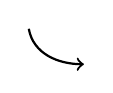
\begin{tikzpicture}
\draw [->,black,line width=0.8] (0,0) to [out=-80,in=180] (0.7,-0.45);
\end{tikzpicture}}
\put(118,-188){
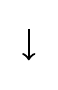
\begin{tikzpicture}
\draw [->,black,line width=0.8] (0,0) to (0,-0.4);
\end{tikzpicture}}

\put(212,-244){

\begin{tikzpicture}
\draw [->,black,line width=0.8] (0,0) to [out=-80,in=180] (0.5,-0.45);
\end{tikzpicture}}
\put(206,-188){
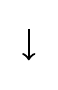
\begin{tikzpicture}
\draw [->,black,line width=0.8] (0,0) to (0,-0.4);
\end{tikzpicture}}
\end{picture}

\begin{picture}(0,0)
\put(90,-260){\liniee{gray}{3}{8.5}}
\end{picture}


\begin{picture}(0,0)
\put(185,-247){\liniee{gray}{3}{8.5}}
\end{picture}

\begin{picture}(0,0)
\put(270,-232){\liniee{gray}{3}{8.5}}
\end{picture}

\vspace{-11px}
%%%%%%%%%%%%%%%%%%%partea de sus

\hspace{-29px}\textit{\textbf{\fontsize{9pt}{0pt}\selectfont{\color{black}Goals:
}}}

%primul dreptughi
\begin{picture}(0,0)
\put(20,0)
{\dreptunghi{1.7cm}{0.6}{
\textbf{\fontsize{6pt}{0pt}\selectfont{\color{black}Articulate:\\
\textbullet who users are \\
\textbullet their key tasks
}}}}
\end{picture}


%dreptughiul 2
\begin{picture}(0,0)
\put(122,15)
{\dreptunghi{1.2cm}{0.6}{
\textbf{\fontsize{6pt}{0pt}\selectfont{\color{black}Brainstorm designs
}}}}
\end{picture}

%dreptughiul 3
\begin{picture}(0,0)
\put(212,30)
{\dreptunghi{1.2cm}{0.2}{
\textbf{\fontsize{6pt}{0pt}\selectfont{\color{black}Refined designs
}}}}
\end{picture}

%dreptughiul 4
\begin{picture}(0,0)
\put(285,42)
{\dreptunghi{1.1cm}{0.2}{
\textbf{\fontsize{6pt}{0pt}\selectfont{\color{gray}Completed designs
}}}}
\end{picture}


\vspace{30px}

%%%%%%%%%%%%%%%%%%%partea de mijloc

\hspace{-29px}\textit{\textbf{\fontsize{8.5pt}{0pt}\selectfont{\color{black}Methods:
}}}


%sageata 1
\vspace{20px}
 \begin{picture}(0,0)
 \put(-4,-12){\sageatainsus{5.5em}{7.4em}{4mm}{1.25cm}{0.4}{\fontsize{6pt}{1pt}\selectfont{\color{black}Task centered system \vspace{4px} design 
Participatory  \vspace{4px} design
User-centered design}}{-90}}
 \end{picture}
 
%sageata 2
 \begin{picture}(0,0)
\put(47,7){\sageatainsus{1.8em}{6.8em}{4.5mm}{0.9cm}{0.6}{\fontsize{6pt}{0pt}\selectfont{\color{black} Evaluate tasks}}{90}}
 \end{picture}


%sageata 3
\begin{picture}(0,0)
\put(90,18){\sageatainsus{5em}{7em}{5mm}{1.3cm}{0.4}{
\textbf{\fontsize{6pt}{0pt}\selectfont{\color{black} Psychology of everyday \vspace{4px}  things}}

\fontsize{6pt}{0pt}\selectfont{\color{black} User \vspace{4px} involvement}

\textbf{\fontsize{6pt}{0pt}\selectfont{\color{red} Representation \& metaphors}}
}{-90}}
 \end{picture}
 
 
 %sageata 3 jos
\begin{picture}(0,0)
\put(90,-20){\sageatainsus{5em}{0em}{5mm}{1.2cm}{0.4}{
\textbf{\fontsize{6pt}{0pt}\selectfont{\color{black} low fidelity prototyping methods}}

}{-90}}
 \end{picture}
 
%sageata 4
\begin{picture}(0,0)
\put(137,50){\sageatainsus{4.5em}{7.4em}{5mm}{1.2cm}{0.4}{

\textit{\fontsize{6pt}{0pt}\selectfont{\color{black} Participatory \vspace{8px} interaction}}

\textit{\fontsize{6pt}{0pt}\selectfont{\color{black} Task scenario walk-through
}}

}{90}}
 \end{picture}

%sageata 5
\begin{picture}(0,0)
\put(185,60){\sageatainsus{4em}{7em}{5mm}{1cm}{0.4}{

\fontsize{6pt}{0pt}\selectfont{\color{gray}Graphical screen  \vspace{4px} design}

\fontsize{6pt}{0pt}\selectfont{\color{gray}Interface \vspace{4px} guidelines}

\fontsize{6pt}{0pt}\selectfont{\color{gray}Style  \vspace{4px} guides}

}{-90}}
 \end{picture}
 
 
 %sageata 5 jos
\begin{picture}(0,0)
\put(185,20){\sageatainsus{5em}{4em}{5mm}{1.2cm}{0.4}{
\textbf{\fontsize{6pt}{0pt}\selectfont{\color{black} high fidelity prototyping methods}}

}{-90}}
 \end{picture}

%sageata 6
\begin{picture}(0,0)
\put(228,88){\sageatainsus{4em}{7em}{5mm}{1cm}{0.4}{

\textit{\fontsize{6pt}{0pt}\selectfont{\color{black} Usability
 \vspace{8px} testing}}

\textit{\fontsize{6pt}{0pt}\selectfont{\color{gray} Heuristic evaluation}}
}{90}}
 \end{picture}

%sageata 7
\begin{picture}(0,0)
\put(296,103){\sageatainsus{2.5em}{7em}{3.6mm}{0.7cm}{0.4}{

\textit{\fontsize{6pt}{0pt}\selectfont{\color{gray}Field testing}}
}{90}}
 \end{picture}
 
 
 
 \vspace{-39px}
 %%%%%%%%%%%%%%%%%%%partea de jos

\hspace{-29px}\vspace{25px}\textit{\textbf{\fontsize{9pt}{0pt}\selectfont{\color{black}Products:
}}}

%dreptunghiul 1
\begin{picture}(0,0)
\put(20,27)
{\dreptunghi{1.4cm}{0.2}{
\textbf{\fontsize{6pt}{0pt}\selectfont{\color{black}User and task descriptions
}}}}
\end{picture}

%dreptunghiul 2
\begin{picture}(0,0)
\put(120,40)
{\dreptunghi{1.4cm}{0.2}{
\textbf{\fontsize{6pt}{0pt}\selectfont{\color{black}Throw-away paper prototypes
}}}}
\end{picture}

%dreptunghiul 3
\begin{picture}(0,0)
\put(205,56)
{\dreptunghi{1.2cm}{0.2}{
\textbf{\fontsize{6pt}{0pt}\selectfont{\color{black}Testable prototypes
}}}}
\end{picture}

%dreptunghiul 4
\begin{picture}(0,0)
\put(280,60)
{\dreptunghi{1.4cm}{0.2}{
\textbf{\fontsize{6pt}{0pt}\selectfont{\color{gray}Alpha/beta systems or complete specification
}}}}
\end{picture}
\end{frame}



{\setbeamercolor{background canvas}{bg=background}
\setbeamercolor{normal text}{fg=blue}
\usebeamercolor[fg]{normal text}
\begin{frame}
{\textbf{*Bibliography}}{\textcolor{red}{\rule{12cm}{1.2pt}}}

        \begin{itemize}
        	\item[{$\bullet$}] Saul Greenberg, \textbf{Designing and building visual interfaces. Representations and information visualization}, University of Calgary, Canada

        	\url{http://pages.cpsc.ucalgary.ca/~saul/481/}
        	\newline
        	 
     	\end{itemize}
\end{frame}



\end{document}